\documentclass[12pt]{article}
\usepackage{graphicx}
\usepackage{amsmath}

\setlength\textwidth{16.0cm}
\setlength\topmargin{-2.5cm}
\setlength\textheight{22.5cm}
\addtolength\evensidemargin{-1.2cm}
\addtolength\oddsidemargin{-1.2cm}
%\addtolength\topmargin{-1.6in}

\newcommand{\half}{{\textstyle\frac{1}{2}}}
\newcommand{\ffrac}[2]{{\textstyle\frac{{#1}}{{#2}}}}
\renewcommand{\tfrac}[2]{{\textstyle\frac{{#1}}{{#2}}}} 

\renewcommand{\topfraction}{0.8}
\renewcommand{\textfraction}{0.2}
\renewcommand{\floatpagefraction}{0.8}



\begin{document}

\title{Radii systematic for various DFT in Ca, Ni, Sn, and Pb chains}
\author{Internal notes: FAU -- MSU}
\date{Started: 11. November 2024}
\maketitle

The archive delivered together with these internal notes contains a
collection of charge r.m.s. radii in the chain of Ca-, Ni-, Sn-, and
Pb-isotopes from proton dripline to neutron dripline (and a bit
beyond) computed with a variety of DFT parametrizations. The results
come in the following files, one separate file for each functional:
\begin{description}
\item{\texttt{collect.SV-min}:}
 \\
 fit Skyrme functional to semi-magic nuclei   \cite{Kluepfel2009} \\[-20pt]
\item{\texttt{collect.SV-min-HFBcut5}} \\
 SV-min where pairing is refitted with HFB \\[-20pt]
\item{\texttt{collect.UNEDF1-BCScut5-rho16}:} \\
 fit Skyrme functional to deformed nuclei, BCS pairing refitted
 \cite{Kortelainen2012}\\[-20pt] 
\item{\texttt{collect.UNEDF1.HFB-rho16}:} \\
  UNEDF1 with HFB pairing refitted\\[-20pt]
\item{\texttt{collect.Fystd}:} \\
Fy(std) = fit Fayans functional to data set of SV-min  \cite{Reinhard2017} \\[-20pt]
\item{\texttt{collect.FyDr}:} \\
Fy($\Delta r$) = extend Fy(std) to include radius differences
in Ca   \cite{Reinhard2017} \\[-20pt]
\item{\texttt{collect.FyDrHFB}:} \\
Fy($\Delta r$,HFB) = extend Fy($\Delta r$)
by data from $^{36}$Ca and use HFB pairing  \cite{Miller2019} \\[-20pt]
\item{\texttt{collect.FyIVP-stab05}:} \\
Fy(IVP) = extend Fy($\Delta r$,HFB) by
different proton-neutron pairing  \cite{Wang2024} \\[-20pt]
\item{\texttt{exp-radii-CaNiSnPb.dat}:} \\
 collection of experimental r.m.s. charge radii 
\end{description}
Supposing that all considered nuclei are spherical, the calculations
were done with a spherical 1D code. The now following figures should
give an impression what the files contain and to address possible
limitations of a spherical mean-field approach.

\begin{figure}[tbp]
\centerline{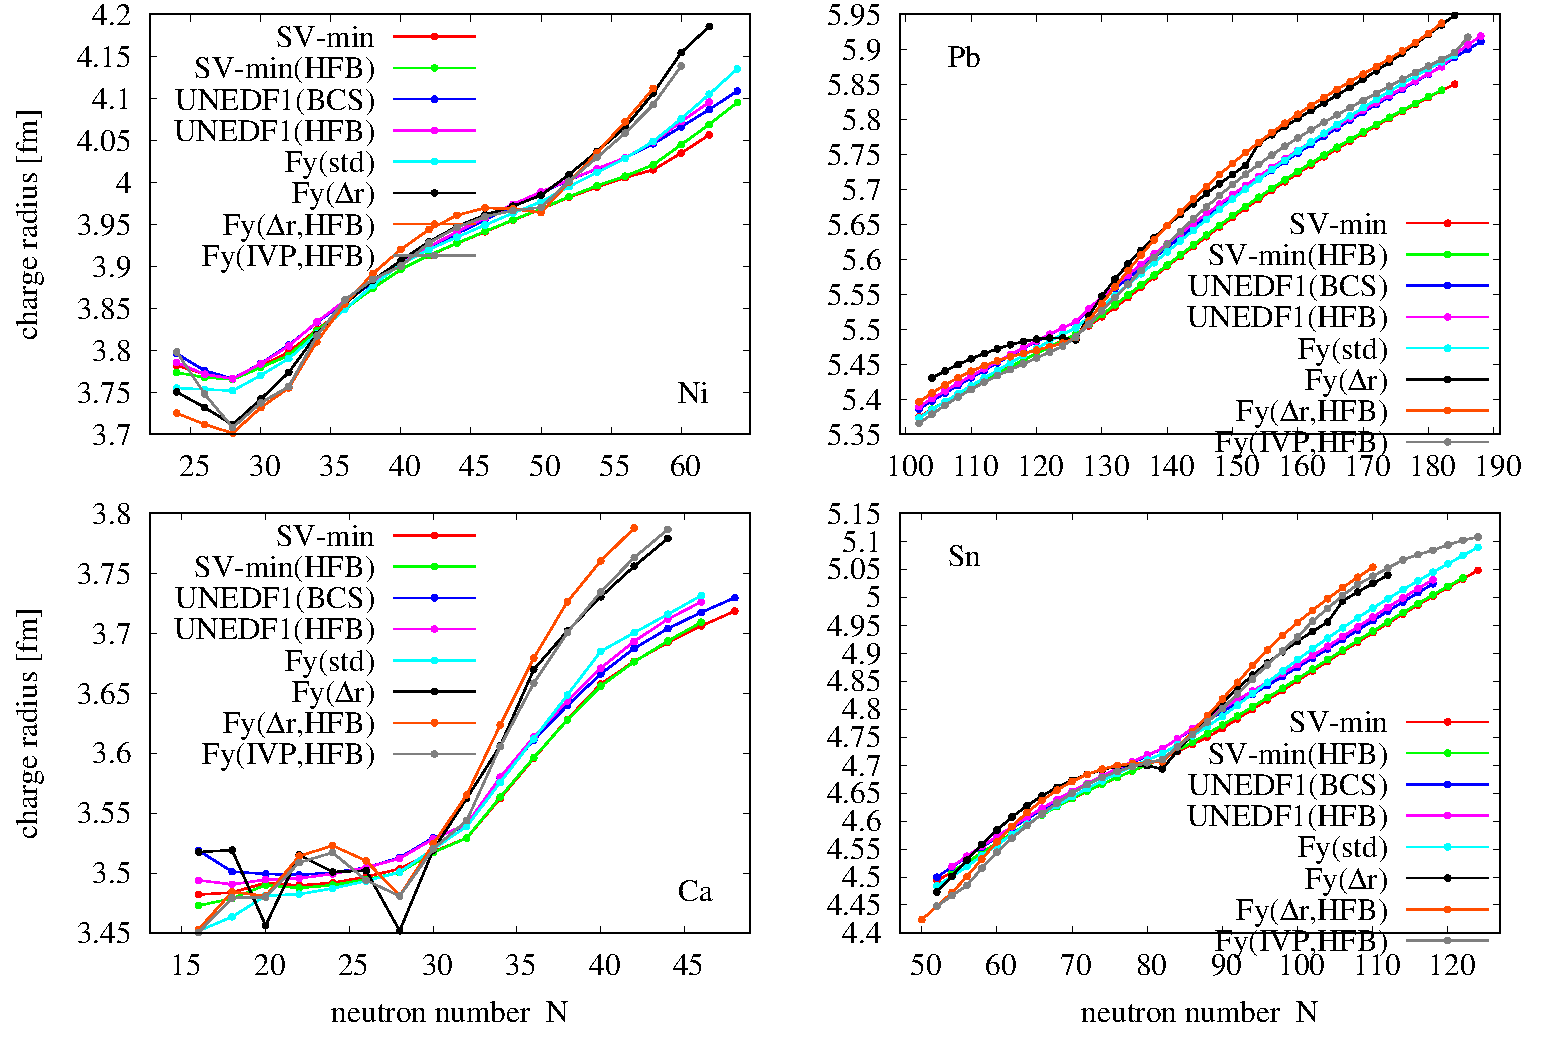
\includegraphics[width=\linewidth]{scan-radii}}
\caption{Charge r.m.s. radii for the four isotopic chains and all DFT
  functionals under consideration. Only result for isotopes within the
  driplines of each DFT have been plotted.}
\label{fig:scan-radii}
\end{figure}
Figure \ref{fig:scan-radii} summarizes all results for the
r.m.s. radii. They separate into two almost distinctive groups of
predictions. At the one side, the four Skyrme functionals plus the
Fayans functional Fy(std), and at the other side, the three remaining
Fayans functionals Fy($\Delta r$), Fy($\Delta r$,HFB), and
Fy(IVP). The latter show a strong enhancement for mid-shell Ca
isotopes in agreement with data (not shown) which is achieved by the
gradient pairing term in the Fayans functional and by including
difference radii in Ca as fit data.

\clearpage

\begin{figure}[tbp]
\centerline{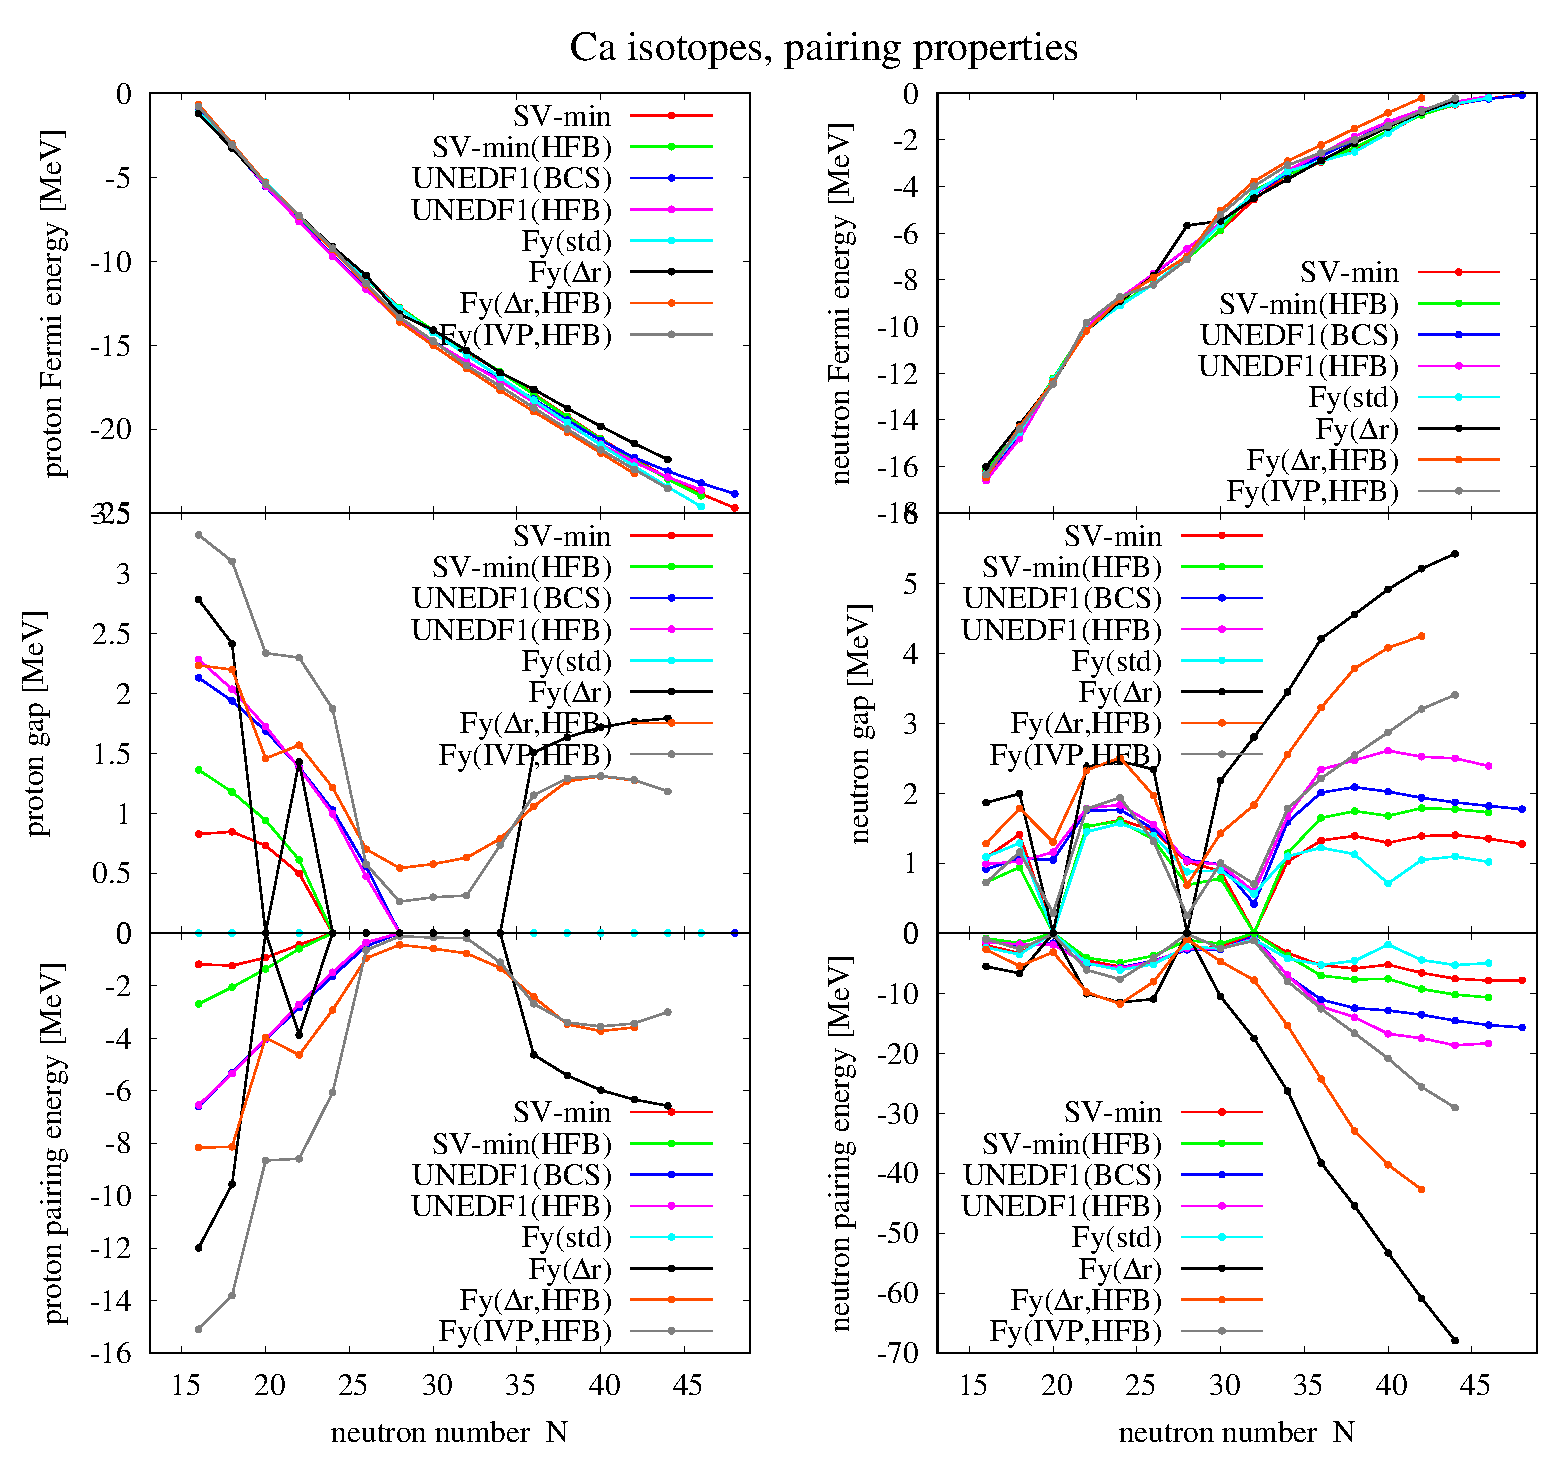
\includegraphics[width=\linewidth]{scan-pairingZ20}}
\caption{Pairing properties (pairing energy, average gap, Fermi
  energy) for protons (left) and neutrons (right) along the chain of
  Ca isotopes for all DFT functionals under consideration. Only result
  for isotopes within the driplines of each DFT have been plotted.}
\label{fig:scan-pairing-Z20}
\end{figure}
Figures \ref{fig:scan-pairing-Z20}--\ref{fig:scan-pairing-Z82} collect
all information on pairing properties.  The Fermi energies (upper
panels) develop with expected trends. Protons are less bound with
shrinking neutron number and neutrons become less bound with
increasing neutron number.  Both trends are terminated with the
respective dripline.  Pairing energies (lower panels) and $u_\alpha
v_\alpha$-averaged pairing gaps (middle panels) contain similar
information with different bias. The gaps indicate how far the
occupation distribution reaches above the Fermi energy. This together
with the position of the Fermi energy allows to estimate the impact
of the continuum. It grows obviously toward both driplines. This puts
a warning sign that mere BCS calculations become unreliable for the
very exotic nuclei near driplines. As a rule-of-thumb, one should be
careful with all isotopes having Fermi energy less than 2 MeV below
continuum threshold. 

It is also interesting to note that proton pairing does not always
vanish although we are dealing with magic proton numbers throughout.
Proton pairing sets is regularly coming up and increasing the farther
away from the regime of stable nuclei.  A minor difference is seen for
Fy($\Delta r$,HFB) and Fy(IVP) which both use stabilized pairing
keeping always some minimal amount of pairing. Thus we see some small
pairing also for stable nuclei. But even here the growth toward
driplines is obvious.
\\

\centerline{\em The discussion is continued with $\hookrightarrow$ figure
  \ref{fig:softness-SVmin} below.}

\begin{figure}[tbp]
\centerline{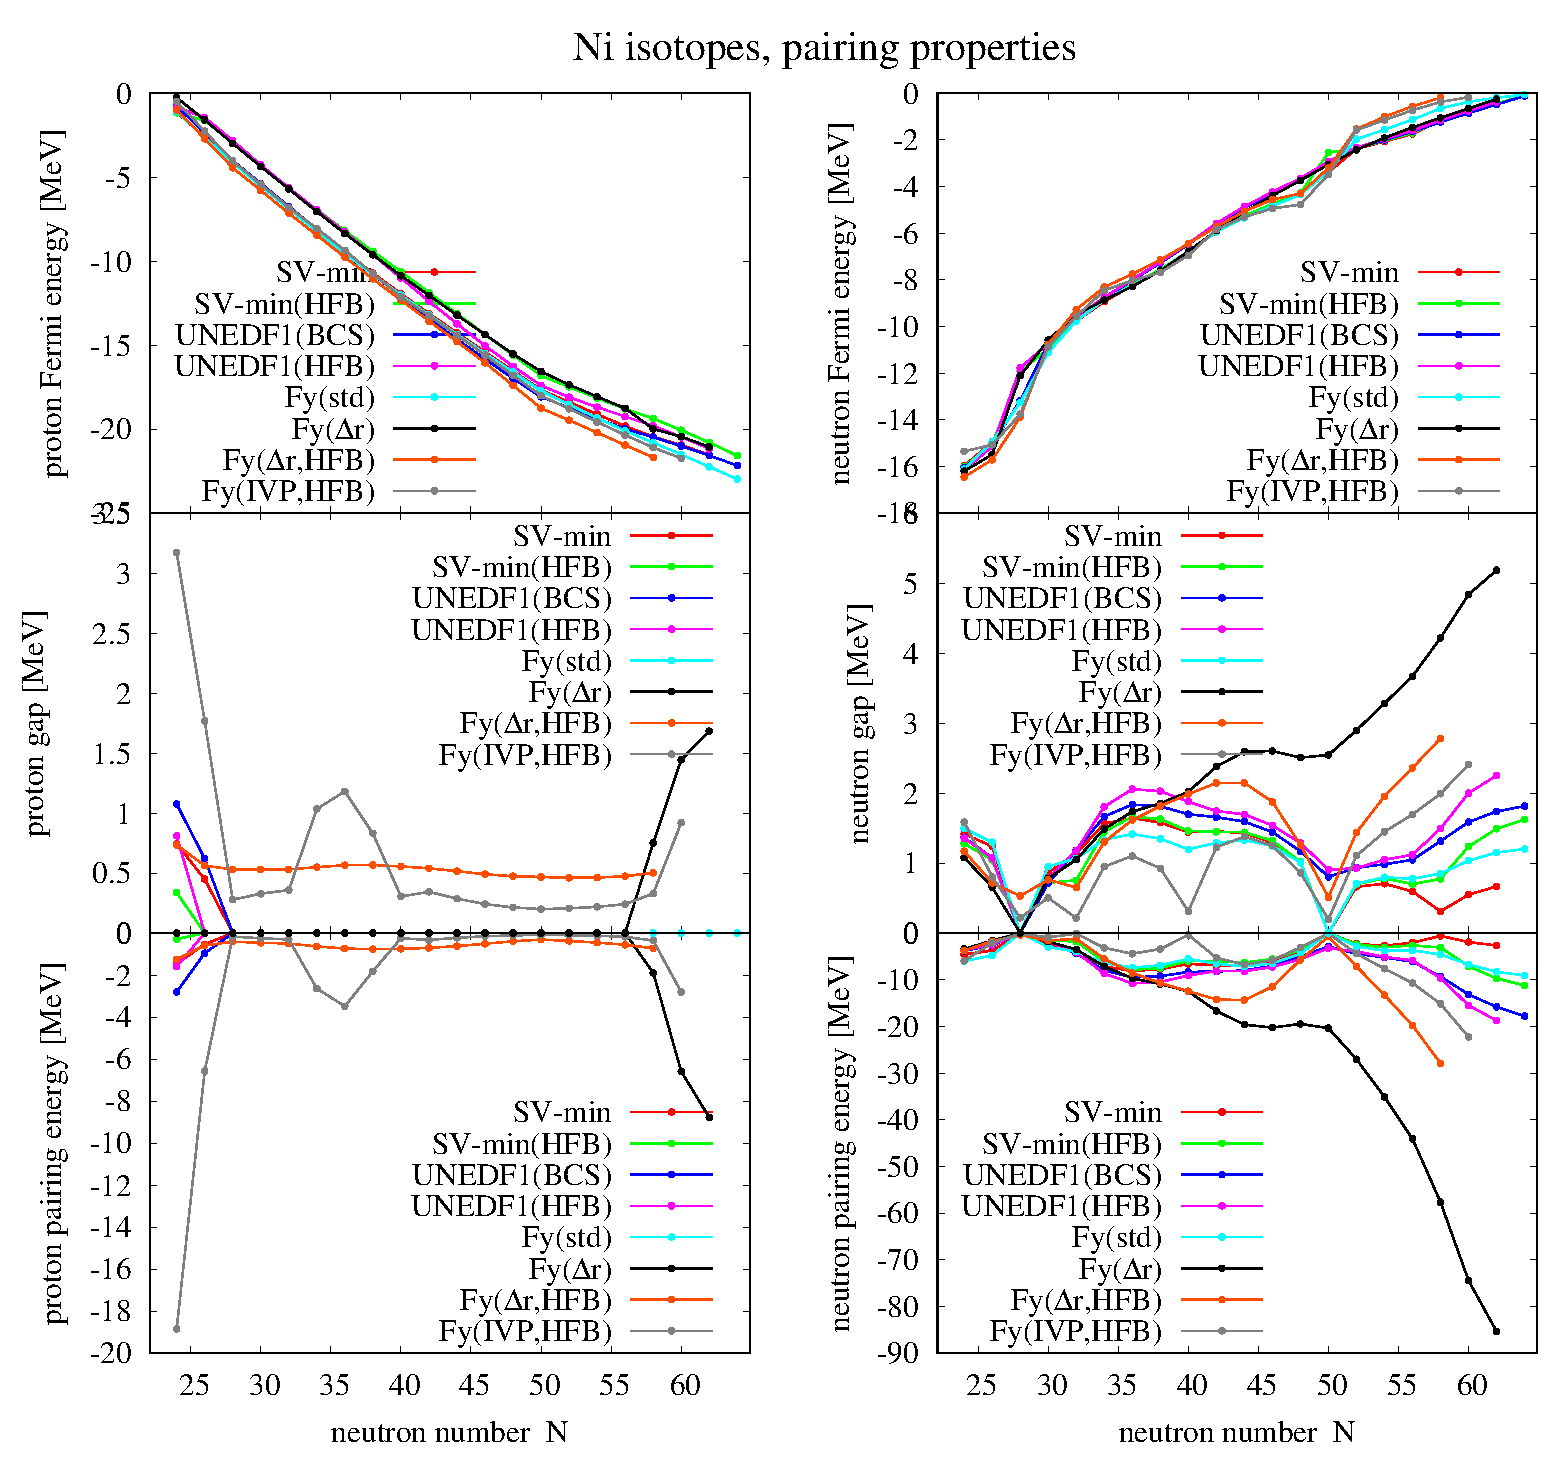
\includegraphics[width=\linewidth]{scan-pairingZ28}}
\caption{Pairing properties (pairing energy, average gap, Fermi
  energy) for protons (left) and neutrons (right) along the chain of
  Ni isotopes for all DFT functionals under consideration. Only result
  for isotopes within the driplines of each DFT have been plotted.}
\label{fig:scan-pairing-Z28}
\end{figure}


\begin{figure}[tbp]
\centerline{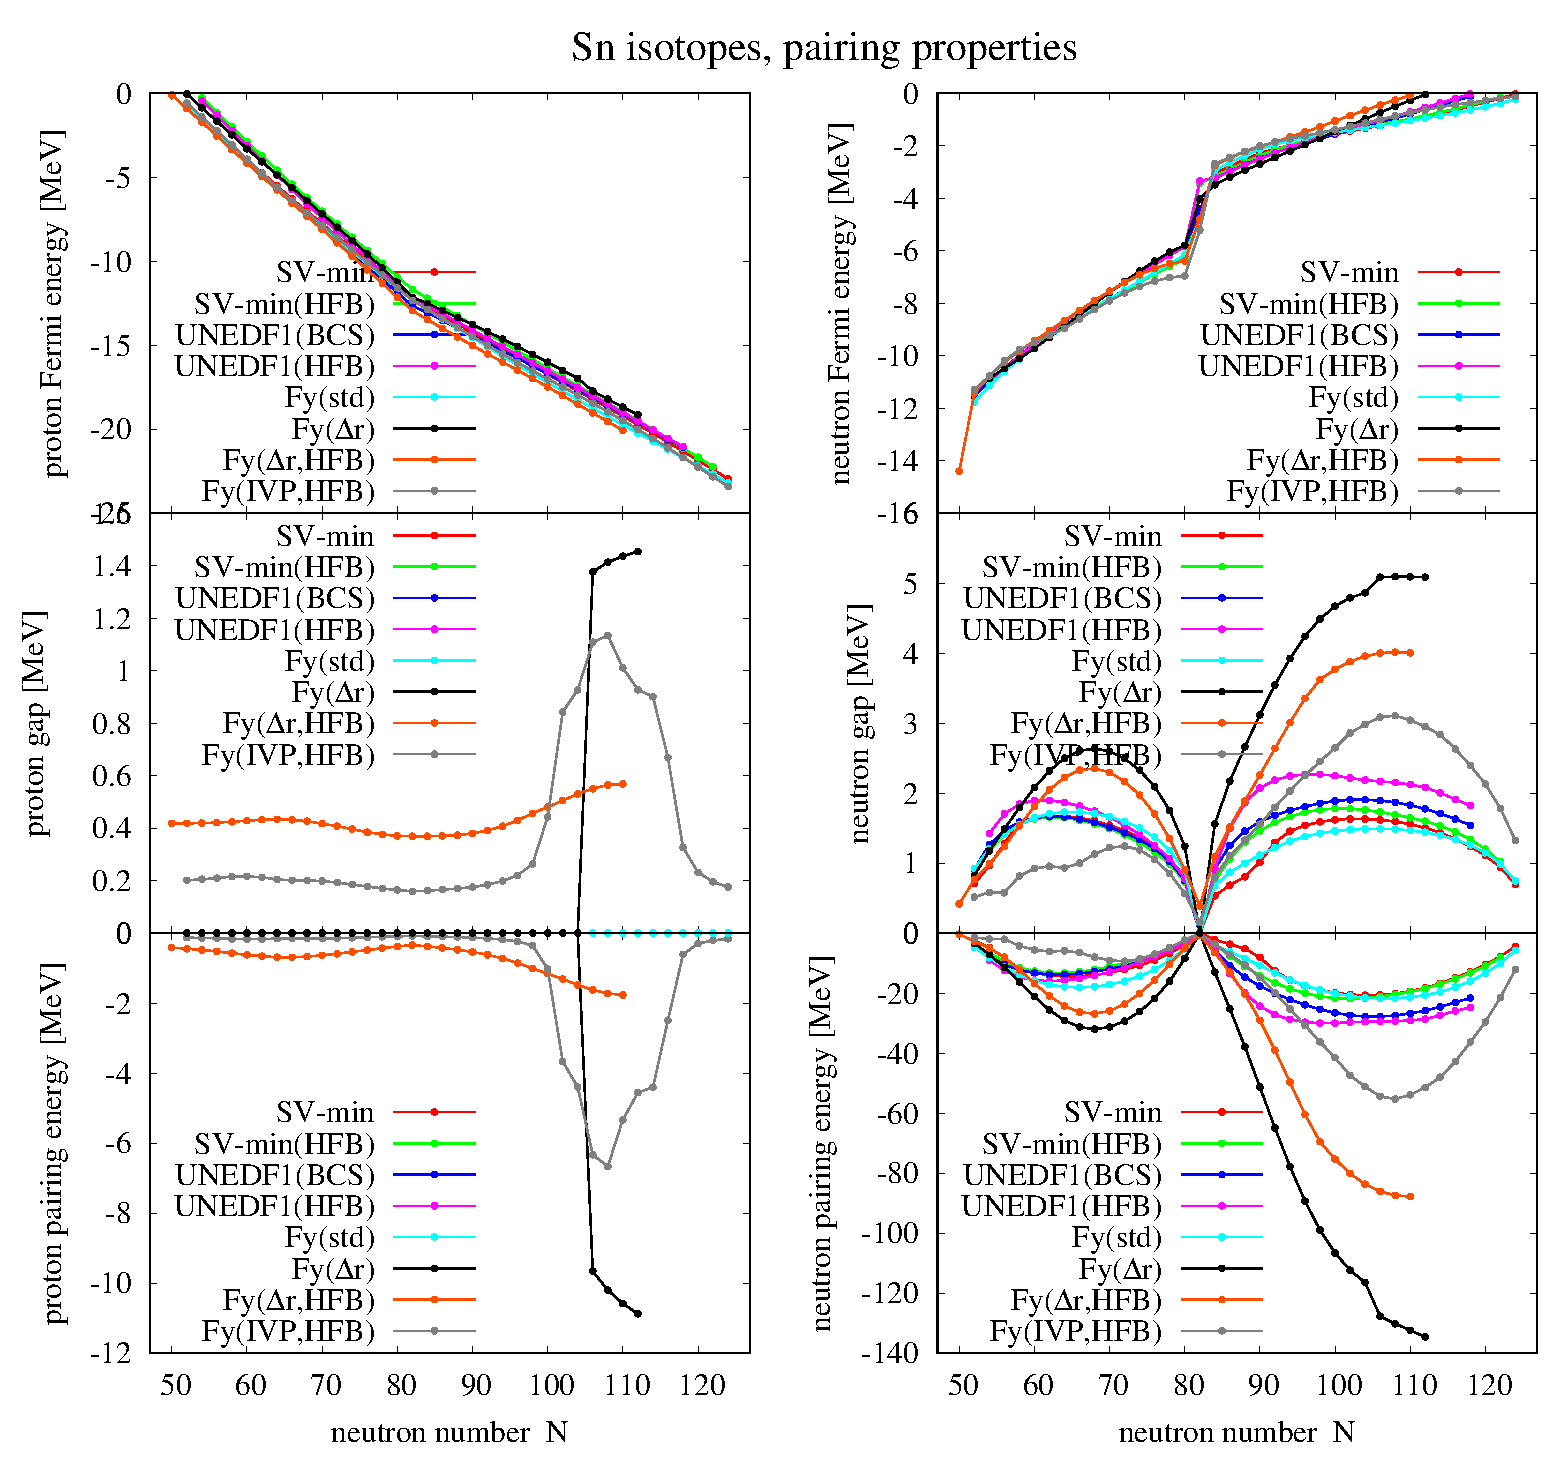
\includegraphics[width=\linewidth]{scan-pairing-Z50}}
\caption{Pairing properties (pairing energy, average gap, Fermi
  energy) for protons (left) and neutrons (right) along the chain of
  Sn isotopes for all DFT functionals under consideration. Only result
  for isotopes within the driplines of each DFT have been plotted.}
\label{fig:scan-pairing-Z50}
\end{figure}


\begin{figure}[tbp]
\centerline{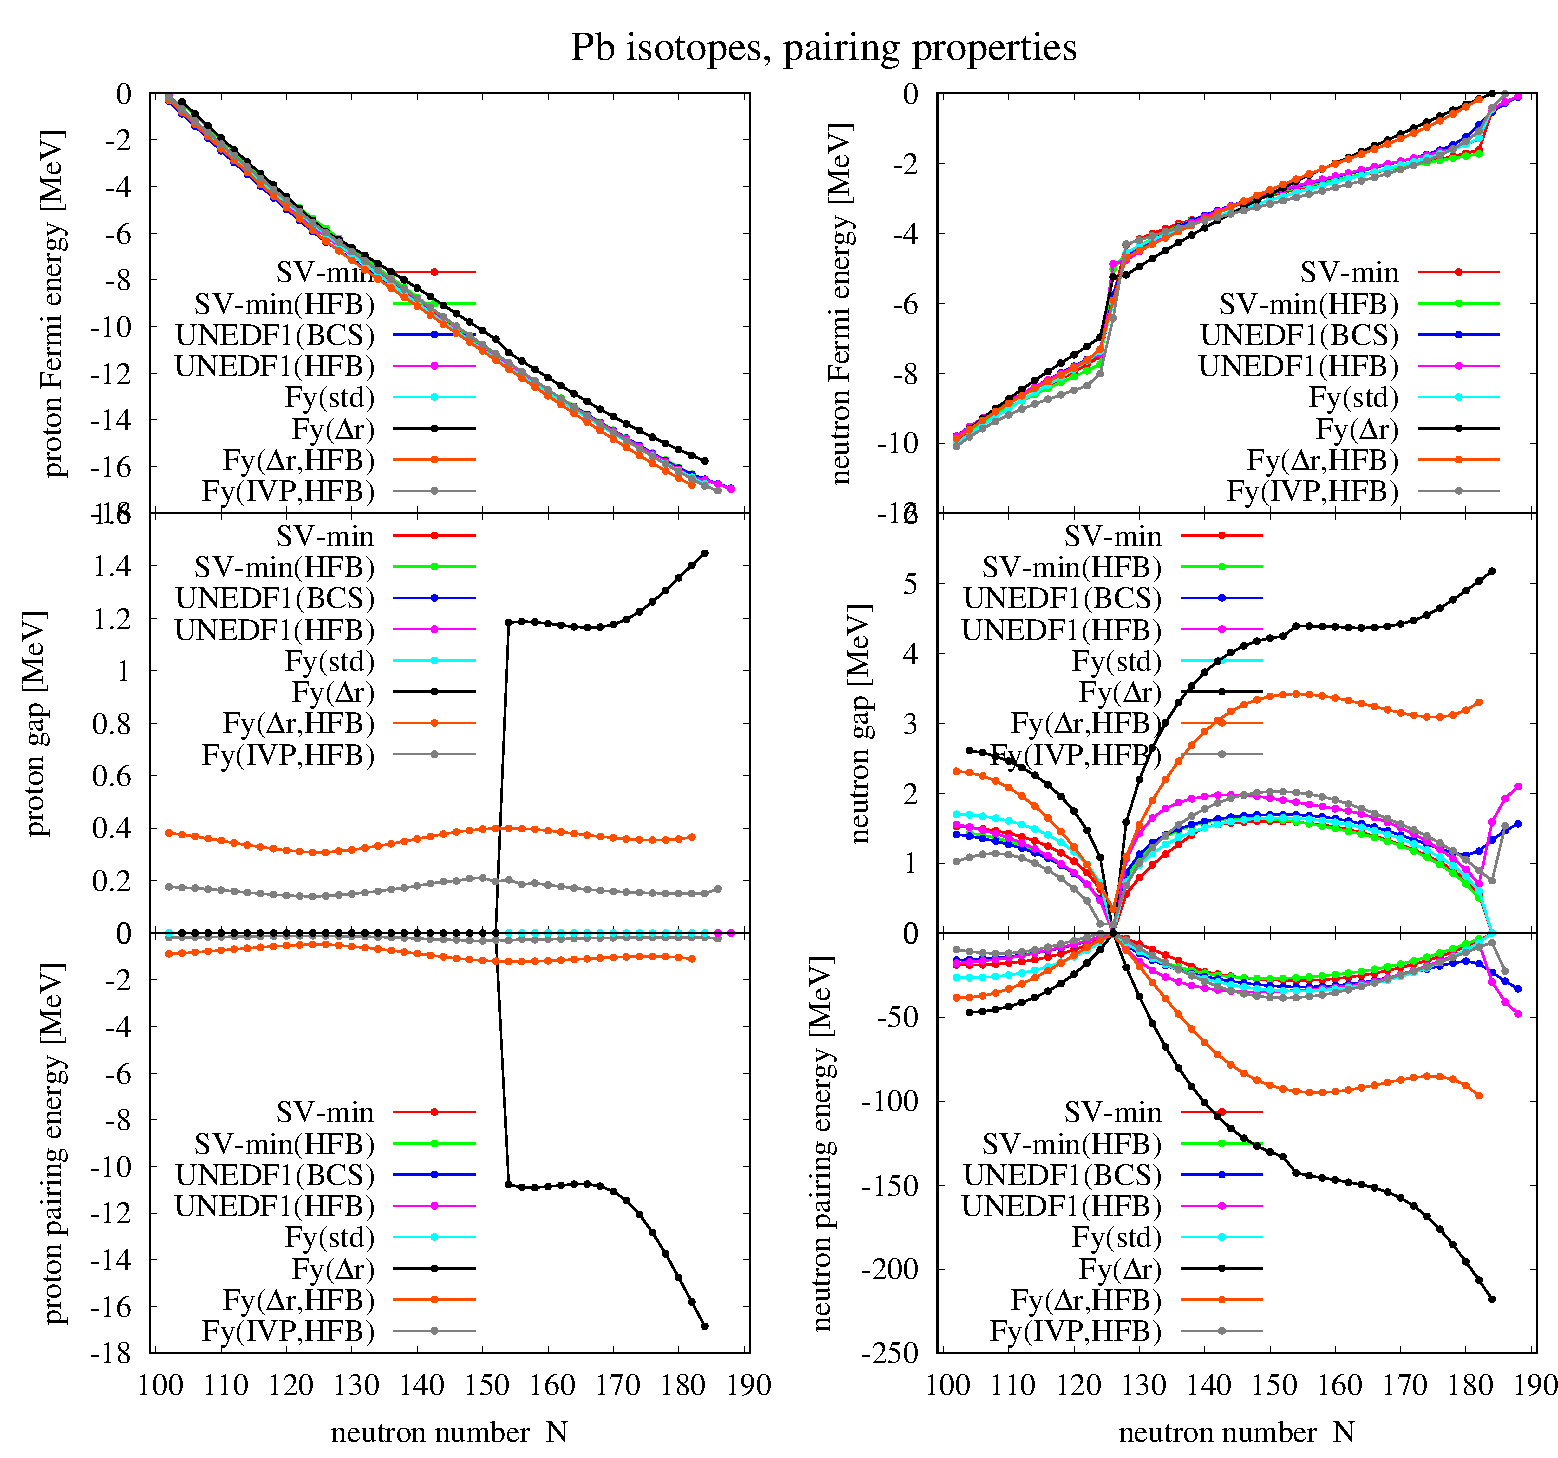
\includegraphics[width=\linewidth]{scan-pairing-Z82}}
\caption{Pairing properties (pairing energy, average gap, Fermi
  energy) for protons (left) and neutrons (right) along the chain of
  Pb isotopes for all DFT functionals under consideration. Only result
  for isotopes within the driplines of each DFT have been plotted.}
\label{fig:scan-pairing-Z82}
\end{figure}


\clearpage

\begin{figure}[tbp]
\centerline{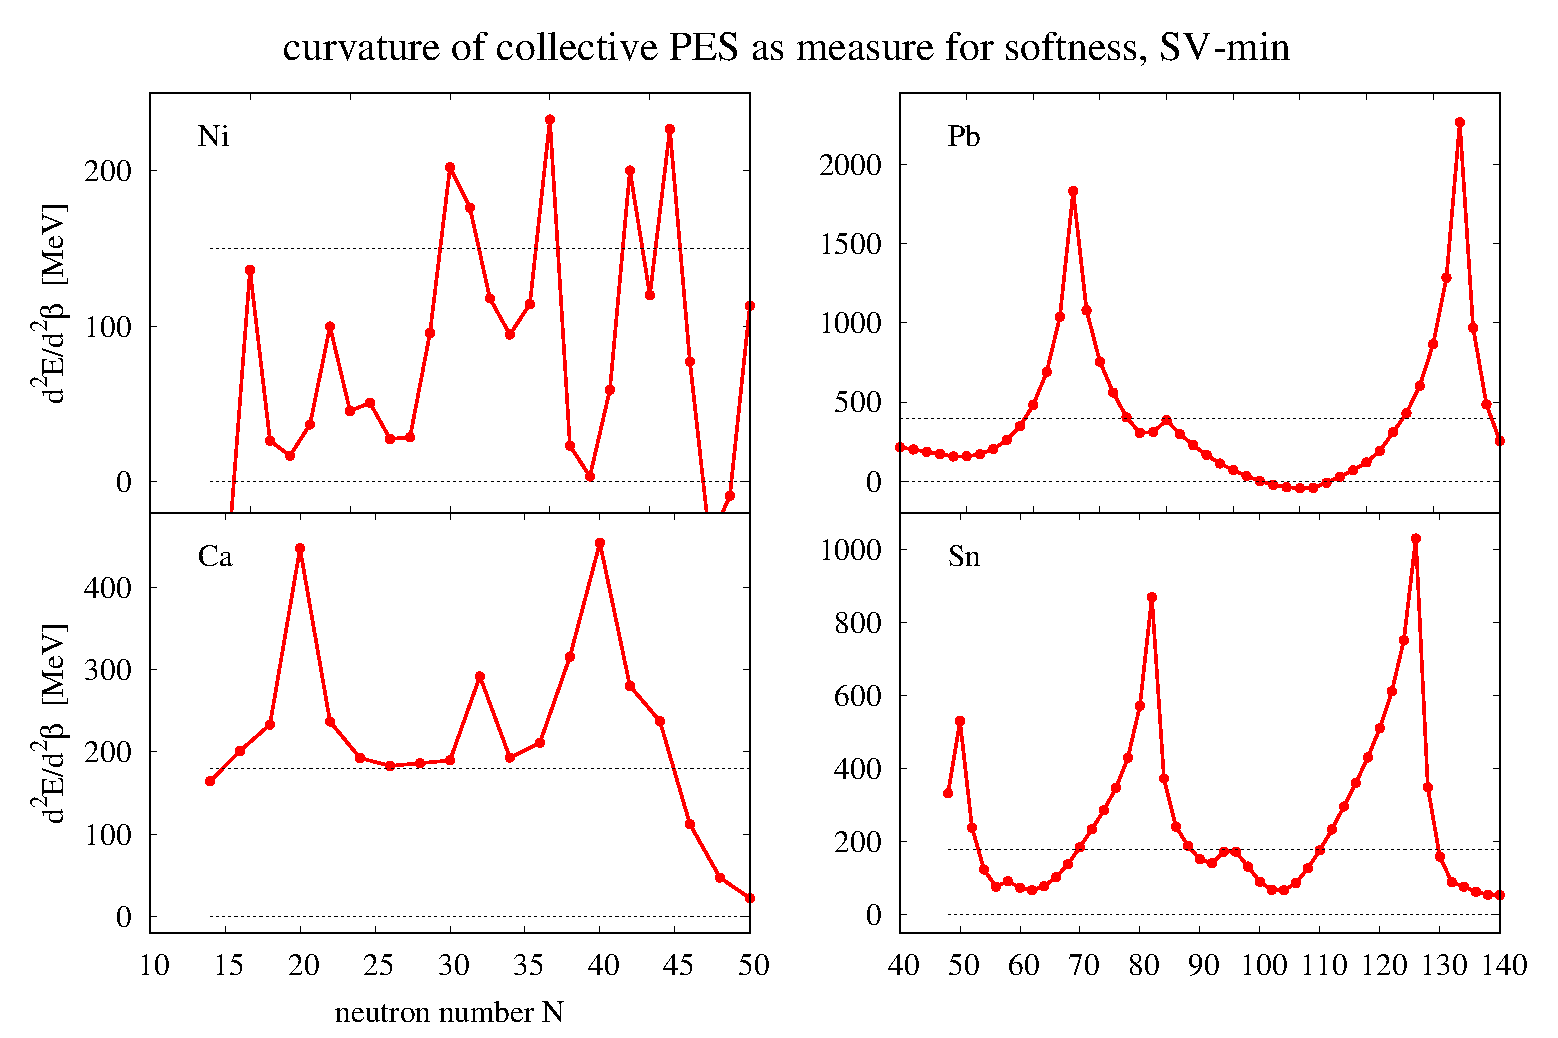
\includegraphics[width=\linewidth]{softness-SVmin}}
\caption{The softness of nuclei estimated from the curvature
$\partial_\beta^2 E(\beta)$ of the collective deformation energy
  $E(\beta)$ at the spherical point. Results computed with SV-min are
shown for the four isotopes under consideration. Each panel contains
two faint horizontal line. One line indicates curvature zero to
distinguish stable spherical minima (positive curvature) from
deformed nuclei. The other horizontal line indicates a ``threshold''
below we which we have to expect considerable correlation corrections 
to the radii. The height of this line is chosen by experience.
}
\label{fig:softness-SVmin}
\end{figure}
Fermi energies close to continuum threshold are one limitation which,
however, applies only when using BCS. There is a more principle
limitation of mean-field calculations coming from collective
vibrational correlations in soft nuclei \cite{Kluepfel2008}. We need
to check that for the present selection of semi-magic isotopic chains.
As a rough measure of softness, we compute the curvature
$\partial_\beta^2 E(\beta)$ of the quadrupole deformation energy
surface. The results are shown in figure
\ref{fig:softness-SVmin}. They are shown only for SV-min. This should
serve to demonstrate general trends. The pattern can change
quantitatively for other functionals.


The maxima at doubly-magic nuclei are obvious. These represent surely
rigid vibrators together with their vicinity. The mean-field
approximation is valid here. Farther away from doubly-magic
configurations the curvature can become suspiciously small. The upper
horizontal faint lines indicate a limit below which experience shows
that correlation corrections to  radii become considerable. This is
also a regime which has to be taken with care.

The lower horizontal line at curvature zero indicates the point below
which spherical nuclei are unstable against deformation. It is
interesting to see that this happens rarely, only for very neutron rich
Pb isotopes. 


%\clearpage

\bibliographystyle{unsrt}
\bibliography{radii-systematic}
\end{document}
